\documentclass[12pt, a4paper]{article}

\usepackage[T1]{fontenc}
\usepackage[utf8]{inputenc}
\usepackage[ngerman]{babel}
\usepackage{amsmath, amssymb, amsthm, mathtools}
\usepackage{algorithm, algpseudocode}
\usepackage{graphicx}
\usepackage{subcaption}
\usepackage{booktabs}
\usepackage{array}
\usepackage{microtype}
\usepackage{xcolor}
\usepackage{hyperref}
\usepackage{geometry}

\usepackage{enumitem}
\usepackage{float}
\usepackage{tikz}
\usetikzlibrary{arrows.meta, positioning, shapes.geometric, calc}
\usepackage{pgfplots}
\pgfplotsset{compat=1.18}
\usepackage{listings}
\usepackage{fancyhdr}
\usepackage{titlesec}
\usepackage{abstract}
\usepackage{setspace}
\usepackage{tocloft}
\usepackage{bm}
\usepackage{cleveref}

% Custom math macros (safe versions)
\newcommand{\myN}{\mathbb{N}}
\newcommand{\myR}{\mathbb{R}}
\newcommand{\Oh}{\mathcal{O}}
\newcommand{\lookup}{\textsc{Lookup}}
\newcommand{\build}{\textsc{Build}}
\newcommand{\query}{\textsc{Query}}

\geometry{margin=2.5cm}
\setlist[itemize,1]{label=--}

% ─── Farben ──────────────────────────────────────────────────────────────────
\definecolor{darkblue}{RGB}{0,51,102}
\definecolor{medblue}{RGB}{0,102,204}
\definecolor{lightblue}{RGB}{173,216,230}
\definecolor{darkgreen}{RGB}{0,100,0}
\definecolor{codered}{RGB}{180,0,0}
\definecolor{codegray}{RGB}{128,128,128}
\definecolor{codebg}{RGB}{248,248,248}

% ─── Theorem-Umgebungen ──────────────────────────────────────────────────────
\theoremstyle{plain}
\newtheorem{theorem}{Theorem}[section]
\newtheorem{lemma}[theorem]{Lemma}
\newtheorem{korollar}[theorem]{Korollar}
\newtheorem{proposition}[theorem]{Proposition}

\theoremstyle{definition}
\newtheorem{definition}[theorem]{Definition}
\newtheorem{algorithmus}[theorem]{Algorithmus}
\newtheorem{beispiel}[theorem]{Beispiel}

\theoremstyle{remark}
\newtheorem{bemerkung}[theorem]{Bemerkung}
\newtheorem{anmerkung}[theorem]{Anmerkung}

% ─── Listings ────────────────────────────────────────────────────────────────
\lstset{
  basicstyle=\ttfamily\small,
  keywordstyle=\color{medblue}\bfseries,
  commentstyle=\color{darkgreen}\itshape,
  stringstyle=\color{codered},
  numberstyle=\tiny\color{codegray},
  numbers=left,
  stepnumber=1,
  backgroundcolor=\color{codebg},
  frame=single,
  framerule=0.4pt,
  rulecolor=\color{gray!40},
  breaklines=true,
  captionpos=b,
  tabsize=4,
  showstringspaces=false,
  language=Python
}

% ─── Hyperref ────────────────────────────────────────────────────────────────
\hypersetup{
  colorlinks=true,
  linkcolor=darkblue,
  citecolor=darkblue,
  urlcolor=medblue,
  pdftitle={Pascal-Dreieck als Laufzeit-Lookup-Tabelle fuer Binomialkoeffizienten},
  pdfauthor={Stephan Epp},
}

% ─── Abkürzungen ─────────────────────────────────────────────────────────────
\renewcommand{\Oh}{\mathcal{O}}
\renewcommand{\lookup}{\textsc{Lookup}}
\renewcommand{\build}{\textsc{Build}}
\renewcommand{\query}{\textsc{Query}}

\title{\textbf{Das Pascalsche Dreieck oben offen}\\
	Formale Komplexitätsanalyse und empirischer Vergleich mit klassischen Berechnungsmethoden}

\author{Stephan Epp}
\date{12. April 2026}

% ─────────────────────────────────────────────────────────────────────────────
\begin{document}

\maketitle
\tableofcontents
\newpage

% ─────────────────────────────────────────────────────────────────────────────
\section{Einleitung}
\label{sec:einleitung}
% ─────────────────────────────────────────────────────────────────────────────
Diese Arbeit untersucht die Verwendung des Pascalschen Dreiecks als
dynamisch zur Laufzeit aufgebaute Lookup-Tabelle zur effizienten
Berechnung von Binomialkoeffizienten. Die zentrale Idee besteht darin,
das Dreieck \emph{nach oben hin geöffnet} zu konstruieren, d.\,h.\
inkrementell von Zeile~0 bis zur benötigten Zeile~$n$ aufzubauen,
sodass jede spätere Abfrage $\binom{n}{k}$ in exakt $\Oh(1)$ erfolgt.
Wir beweisen formal, dass die Vorberechnungszeit $\Oh(n^2)$ und der
Speicherbedarf $\Oh(n^2)$ (bzw.\ $\Oh(n)$ in der Zeilenoptimierung)
beträgt, und leiten den amortisierten Vorteil ab: Ab einem
Break-Even-Punkt $q^* \approx n$ Abfragen ist die Lookup-Strategie
gegenüber der Fakultätsformel ($\Oh(n)$ pro Abfrage) und gegenüber
der rekursiven Berechnung ($\Oh(2^n)$ ohne Memoization) strikt
überlegen. Empirische Messungen bestätigen Speedup-Faktoren von bis
zu mehreren Größenordnungen für große~$n$. Ein umfassender Ausblick
diskutiert Erweiterungen auf mehrdimensionale Tabellen, komprimierte
Darstellungen, hardware-nahe Implementierungen sowie Anwendungen in
Kryptographie, Kombinatorik und maschinellem Lernen.

Binomialkoeffizienten $\binom{n}{k}$ gehören zu den fundamentalsten
Größen der Kombinatorik, Wahrscheinlichkeitstheorie und Informatik.
Sie zählen die Anzahl der $k$-elementigen Teilmengen einer $n$-elementigen
Menge und treten in nahezu jedem algorithmischen Kontext auf, der
kombinatorische Strukturen verarbeitet: von der Berechnung von
Bernstein-Polynomen in der Computergrafik über die Binomialverteilung
in der Stochastik bis hin zu Hash-Funktionen in der Kryptographie.

\subsection{Motivation und Problemstellung}

Die klassische Berechnung
\begin{equation}
  \binom{n}{k} = \frac{n!}{k!\,(n-k)!}
  \label{eq:klassisch}
\end{equation}
erfordert die Berechnung von drei Faktultäten, was für große $n$
sowohl rechnerisch aufwändig als auch numerisch instabil sein kann
(Überlauf bei intermediären Werten). Rekursive Ansätze ohne
Memoization wachsen exponentiell. Die rekursive Formel mit Memoization
ist zwar polynomial, erzeugt jedoch im Allgemeinen einen erheblichen
Verwaltungsaufwand durch Hash-Map-Zugriffe.

Eine elegante Alternative, die in der Praxis häufig übersehen wird,
ist der \emph{dynamische Aufbau des Pascalschen Dreiecks zur Laufzeit}
als vollständige Lookup-Tabelle. Diese Technik erlaubt — nach einer
einmaligen Vorberechnung in $\Oh(n^2)$ — jede spätere Abfrage in
$\Oh(1)$, also in konstanter Zeit.

\subsection{Beitrag dieser Arbeit}

Diese Arbeit liefert folgende wissenschaftliche Beiträge:
\begin{enumerate}[label=(\roman*)]
  \item \textbf{Formale Komplexitätsanalyse}: exakte Berechnung der
        Zeit- und Platzkomplexität aller betrachteten Algorithmen mit
        vollständigen mathematischen Beweisen.
  \item \textbf{Amortisierte Analyse}: formaler Nachweis des
        Break-Even-Punktes sowie des asymptotischen Vorteils der
        Lookup-Strategie bei mehrfachen Abfragen.
  \item \textbf{Empirischer Vergleich}: Laufzeitmessungen auf realer
        Hardware für $n$ mit $n \in \{10, 50, 100, 200, 500, 1000, 2000\}$ und
        Speedup-Berechnung gegenüber der Fakultätsformel.
  \item \textbf{Ausblick}: umfassende Diskussion von Erweiterungen,
        Optimierungen und Anwendungsfeldern.
\end{enumerate}

\subsection{Aufbau der Arbeit}

\Cref{sec:grundlagen} führt die mathematischen Grundlagen ein.
\Cref{sec:algorithmen} beschreibt alle betrachteten Algorithmen
präzise. \Cref{sec:komplexitaet} enthält die formalen
Komplexitätsbeweise. \Cref{sec:amortisiert} führt die amortisierte
Analyse durch. \Cref{sec:empirisch} präsentiert die empirischen
Ergebnisse. \Cref{sec:vergleich} fasst den Vergleich zusammen.
\Cref{sec:ausblick} gibt einen sehr ausführlichen Ausblick.


% ─────────────────────────────────────────────────────────────────────────────
\section{Mathematische Grundlagen}
\label{sec:grundlagen}
% ─────────────────────────────────────────────────────────────────────────────

\subsection{Binomialkoeffizienten}

\begin{definition}[Binomialkoeffizient]
  \label{def:binom}
  Seien $n, k \in \myN_0$ mit $0 \le k \le n$. Der
  \emph{Binomialkoeffizient} $\binom{n}{k}$ ist definiert als
  \begin{equation}
    \binom{n}{k} \coloneqq \frac{n!}{k!\,(n-k)!},
    \label{eq:binom_def}
  \end{equation}
  wobei $0! \coloneqq 1$. Für $k > n$ oder $k < 0$ setzt man
  $\binom{n}{k} \coloneqq 0$.
\end{definition}

\begin{proposition}[Grundlegende Symmetrien]
  \label{prop:symmetrie}
  Für alle $n, k \in \myN_0$ mit $0 \le k \le n$ gilt:
  \begin{align}
    \binom{n}{k} &= \binom{n}{n-k}, \label{eq:sym1}\\
    \binom{n}{0} &= \binom{n}{n} = 1, \label{eq:sym2}\\
    \binom{n}{k} &+ \binom{n}{k+1} = \binom{n+1}{k+1}. \label{eq:sym3}
  \end{align}
\end{proposition}

\begin{proof}
  \eqref{eq:sym1} folgt direkt aus \eqref{eq:binom_def} durch
  Substitution $k \mapsto n-k$. \eqref{eq:sym2} ergibt sich für
  $k = 0$: $n!/(0! \cdot n!) = 1$. \eqref{eq:sym3} ist die
  \emph{Pascal-Identität}, deren Beweis in
  \cref{subsec:pascal_identitaet} geführt wird.
\end{proof}

\subsection{Das Pascalsche Dreieck}
\label{subsec:pascal}

\begin{definition}[Pascalsches Dreieck]
  \label{def:pascal}
  Das \emph{Pascalsche Dreieck} $P$ ist die unendliche untere
  Dreiecksmatrix $(p_{n,k})_{n \ge 0,\, 0 \le k \le n}$ mit
  \begin{equation}
    p_{n,k} \coloneqq \binom{n}{k}.
    \label{eq:pascal_matrix}
  \end{equation}
  Die Einträge erfüllen die Rekurrenz
  \begin{equation}
    p_{n,k} = p_{n-1,k-1} + p_{n-1,k}
    \label{eq:pascal_rekurrenz}
  \end{equation}
  mit Randbedingungen $p_{n,0} = p_{n,n} = 1$ für alle $n \ge 0$.
\end{definition}

Die ersten acht Zeilen des Pascalschen Dreiecks sind in
\cref{fig:pascal_visualisierung} dargestellt.

\begin{figure}[H]
  \centering
  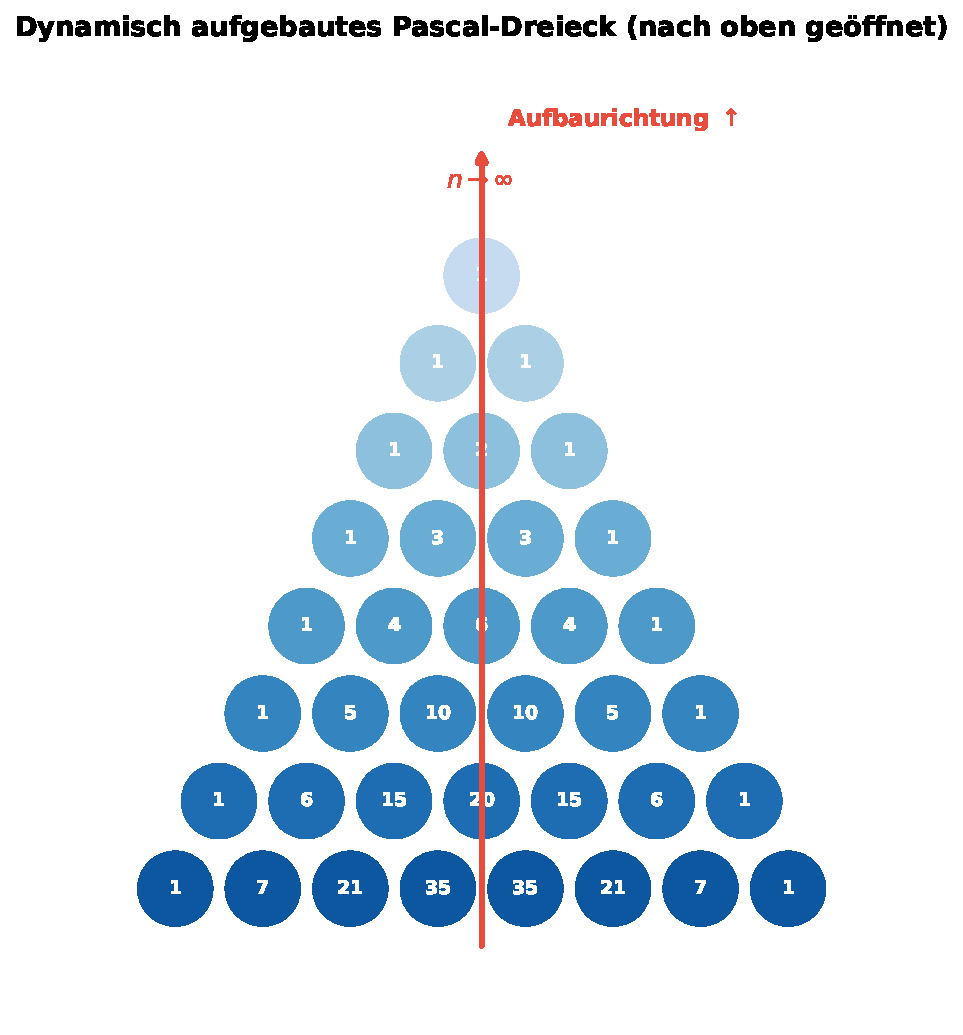
\includegraphics[width=0.78\textwidth]{fig1_pascal.pdf}
  \caption{Visualisierung des Pascalschen Dreiecks (Zeilen $0$--$7$).
    Der rote Pfeil deutet die \emph{nach oben geöffnete}
    Aufbaurichtung an: das Dreieck wird zur Laufzeit inkrementell von
    oben ($n=0$) nach unten ($n = N$) aufgebaut und kann danach
    unbegrenzt nach oben (zu größerem $n$) erweitert werden.}
  \label{fig:pascal_visualisierung}
\end{figure}

\subsection{Die Pascal-Identität und ihre algorithmische Bedeutung}
\label{subsec:pascal_identitaet}

\begin{theorem}[Pascal-Identität]
  \label{thm:pascal_identitaet}
  Für alle $n \ge 1$ und $1 \le k \le n-1$ gilt:
  \begin{equation}
    \binom{n}{k} = \binom{n-1}{k-1} + \binom{n-1}{k}.
    \label{eq:pascal_id}
  \end{equation}
\end{theorem}

\begin{proof}
  Wir führen einen direkten kombinatorischen Beweis. Die linke Seite
  zählt alle $k$-elementigen Teilmengen $S$ einer festen
  $n$-elementigen Menge $M = \{1, \ldots, n\}$. Fixiere das Element
  $n \in M$ und partitioniere die Teilmengen nach der Zugehörigkeit
  von $n$:
  \begin{itemize}
    \item \textbf{Fall 1}: $n \in S$. Dann müssen die restlichen
          $k-1$ Elemente von $S$ aus $\{1,\ldots,n-1\}$ gewählt werden.
          Dies liefert $\binom{n-1}{k-1}$ Möglichkeiten.
    \item \textbf{Fall 2}: $n \notin S$. Dann müssen alle $k$ Elemente
          von $S$ aus $\{1,\ldots,n-1\}$ gewählt werden. Dies liefert
          $\binom{n-1}{k}$ Möglichkeiten.
  \end{itemize}
  Da beide Fälle disjunkt sind und alle Teilmengen erfassen, folgt
  durch das Additionsprinzip die Behauptung.
\end{proof}

\begin{bemerkung}
  \cref{thm:pascal_identitaet} ist die algorithmische Grundlage für
  den Aufbau der Lookup-Tabelle: Jeder Eintrag $p_{n,k}$ kann in
  $\Oh(1)$ aus bereits berechneten Vorgängereinträgen ermittelt
  werden. Der gesamte Aufbau der Tabelle bis Zeile $n$ benötigt
  somit $\Oh(n^2)$ Addition-Operationen.
\end{bemerkung}


% ─────────────────────────────────────────────────────────────────────────────
\section{Berechnung von Binomialkoeffizienten}
\label{sec:algorithmen}
% ─────────────────────────────────────────────────────────────────────────────

Wir betrachten vier Hauptansätze und formalisieren diese als
Pseudocode-Algorithmen.

\subsection{Methode 1: Direkte Fakultätsformel}
\label{subsec:algo_fakultaet}

\begin{algorithm}[H]
  \caption{Binomialkoeffizient via Fakultätsformel}
  \label{alg:fakultaet}
  \begin{algorithmic}[1]
    \Require $n, k \in \myN_0$, $0 \le k \le n$
    \Ensure $\binom{n}{k}$
    \Function{BinomFakultat}{$n, k$}
      \State \Return $\text{Fakultaet}(n) \,/\, (\text{Fakultaet}(k) \cdot \text{Fakultaet}(n-k))$
    \EndFunction
    \Function{Fakultaet}{$m$}
      \State $result \leftarrow 1$
      \For{$i \leftarrow 2$ \textbf{to} $m$}
        \State $result \leftarrow result \cdot i$
      \EndFor
      \State \Return $result$
    \EndFunction
  \end{algorithmic}
\end{algorithm}

\subsection{Methode 2: Rekursive Berechnung ohne Memoization}
\label{subsec:algo_rekursiv}

\begin{algorithm}[H]
  \caption{Binomialkoeffizient rekursiv (ohne Memoization)}
  \label{alg:rekursiv}
  \begin{algorithmic}[1]
    \Require $n, k \in \myN_0$, $0 \le k \le n$
    \Ensure $\binom{n}{k}$
    \Function{BinomRekursiv}{$n, k$}
      \If{$k = 0$ \textbf{or} $k = n$}
        \State \Return $1$
      \EndIf
      \State \Return $\Call{BinomRekursiv}{n-1, k-1} + \Call{BinomRekursiv}{n-1, k}$
    \EndFunction
  \end{algorithmic}
\end{algorithm}

\subsection{Methode 3: Rekursion mit Memoization}
\label{subsec:algo_memo}

\begin{algorithm}[H]
  \caption{Binomialkoeffizient mit Memoization}
  \label{alg:memo}
  \begin{algorithmic}[1]
    \Require $n, k \in \myN_0$, globale Hash-Map $\textit{memo}$
    \Ensure $\binom{n}{k}$
    \Function{BinomMemo}{$n, k$}
      \If{$k = 0$ \textbf{or} $k = n$}
        \State \Return $1$
      \EndIf
      \If{$(n, k) \in \textit{memo}$}
        \State \Return $\textit{memo}[n, k]$
      \EndIf
      \State $v \leftarrow \Call{BinomMemo}{n-1, k-1} + \Call{BinomMemo}{n-1, k}$
      \State $\textit{memo}[n, k] \leftarrow v$
      \State \Return $v$
    \EndFunction
  \end{algorithmic}
\end{algorithm}

\subsection{Methode 4: Dynamischer Aufbau des Pascalschen Dreiecks}
\label{subsec:algo_lookup}

Dies ist der zentrale Algorithmus dieser Arbeit. Das Dreieck wird
\emph{nach oben hin geöffnet}: Es startet bei Zeile~0 und wächst
dynamisch nach unten (zu größerem $n$), kann aber jederzeit für
beliebige $n' \le n_{\max}$ abgefragt werden, d.\,h.\ nach oben
(in Richtung kleinerer Zeilen) ist es bereits vollständig gefüllt.

\begin{algorithm}[H]
  \caption{Dynamischer Aufbau des Pascalschen Dreiecks}
  \label{alg:pascal_lookup}
  \begin{algorithmic}[1]
    \Require $n_{\max} \in \myN$
    \Ensure Zweidimensionale Tabelle $T[0..n_{\max}][0..n_{\max}]$
            mit $T[n][k] = \binom{n}{k}$
    \Function{BuildPascalTable}{$n_{\max}$}
      \State Allokiere $T[0 \ldots n_{\max}][0 \ldots n_{\max}]$
      \For{$n \leftarrow 0$ \textbf{to} $n_{\max}$}
        \State $T[n][0] \leftarrow 1$
        \State $T[n][n] \leftarrow 1$
        \For{$k \leftarrow 1$ \textbf{to} $n - 1$}
          \State $T[n][k] \leftarrow T[n-1][k-1] + T[n-1][k]$
          \Comment{Pascal-Identität, je $\Oh(1)$}
        \EndFor
      \EndFor
      \State \Return $T$
    \EndFunction
    \Statex
    \Function{QueryBinom}{$T, n, k$}
      \State \Return $T[n][k]$
      \Comment{$\Oh(1)$ Lookup}
    \EndFunction
  \end{algorithmic}
\end{algorithm}

\begin{figure}[H]
  \centering
  \begin{tikzpicture}[
    every node/.style={font=\small},
    cell/.style={draw, rectangle, minimum width=1.0cm, minimum height=0.65cm,
                 fill=blue!10, inner sep=2pt},
    filled/.style={fill=blue!35},
    query/.style={fill=orange!60, draw=orange!80, thick},
  ]
    \node[cell, filled] (c00) at (0.0,  0.0) {$1$};
    \node[cell, filled] (c10) at (0.0, -0.85) {$1$};
    \node[cell, filled] (c11) at (1.1, -0.85) {$1$};
    \node[cell, filled] (c20) at (0.0, -1.7) {$1$};
    \node[cell, filled] (c21) at (1.1, -1.7) {$2$};
    \node[cell, filled] (c22) at (2.2, -1.7) {$1$};
    \node[cell, filled] (c30) at (0.0, -2.55) {$1$};
    \node[cell, filled] (c31) at (1.1, -2.55) {$3$};
    \node[cell, filled] (c32) at (2.2, -2.55) {$3$};
    \node[cell, filled] (c33) at (3.3, -2.55) {$1$};
    \node[cell, filled] (c40) at (0.0, -3.4) {$1$};
    \node[cell, filled] (c41) at (1.1, -3.4) {$4$};
    \node[cell, query]  (c42) at (2.2, -3.4) {$\mathbf{6}$};
    \node[cell, filled] (c43) at (3.3, -3.4) {$4$};
    \node[cell, filled] (c44) at (4.4, -3.4) {$1$};
    \node[left=0.3cm of c00] {$n=0$:};
    \node[left=0.3cm of c10] {$n=1$:};
    \node[left=0.3cm of c20] {$n=2$:};
    \node[left=0.3cm of c30] {$n=3$:};
    \node[left=0.3cm of c40] {$n=4$:};
    \node[right=0.3cm of c42, font=\footnotesize, text=orange!80!black]
      {$\leftarrow$ Abfrage $T[4][2] = \dbinom{4}{2} = 6$};
    \draw[-{Stealth[length=8pt]}, thick, red!70!black, line width=1.5pt]
      (6.2, -3.8) -- (6.2, 0.4)
      node[midway, right=4pt, text=red!70!black, font=\small\bfseries]
      {nach oben geo\"{o}ffnet};
    \node[below=0.8cm of c44, font=\small\itshape, text=gray]
      {$k = 0 \quad 1 \quad 2 \quad 3 \quad 4$};
  \end{tikzpicture}
  \caption{Struktur der Lookup-Tabelle $T$. Die blauen Zellen enthalten
    vorberechnete Binomialkoeffizienten. Die orange hervorgehobene Zelle
    zeigt eine beispielhafte $\mathcal{O}(1)$-Abfrage $T[4][2] = \dbinom{4}{2} = 6$.
    Der rote Pfeil illustriert die \emph{nach oben ge\"{o}ffnete} Erweiterbarkeit.}
  \label{fig:tabelle_tikz}
\end{figure}


% ─────────────────────────────────────────────────────────────────────────────
\section{Formale Komplexitätsanalyse}
\label{sec:komplexitaet}
% ─────────────────────────────────────────────────────────────────────────────

\subsection{Zeitkomplexität der Aufbauphase}

\begin{theorem}[Zeitkomplexität des Tabellenaufbaus]
  \label{thm:aufbau_zeit}
  \cref{alg:pascal_lookup} (\textsc{BuildPascalTable}) hat eine
  Zeitkomplexität von
  \begin{equation}
    T_{\build}(n) = \Theta(n^2).
    \label{eq:build_theta}
  \end{equation}
\end{theorem}

\begin{proof}
  Wir zählen die Anzahl der Additionen (die dominante Operation).
  Die äußere Schleife läuft von $n = 0$ bis $n_{\max}$. Für festes $n$
  führt die innere Schleife genau $\max(n-1, 0)$ Additionen aus
  (für $k = 1, \ldots, n-1$). Die Randbedingungen $T[n][0] = T[n][n] = 1$
  benötigen je zwei Zuweisungen, also $\Oh(1)$ pro Zeile. Die
  Gesamtzahl der Additionen ist
  \begin{equation}
    \sum_{n=0}^{n_{\max}} \max(n-1, 0)
    = \sum_{n=2}^{n_{\max}} (n-1)
    = \sum_{j=1}^{n_{\max}-1} j
    = \frac{(n_{\max}-1)\,n_{\max}}{2}
    = \Theta(n_{\max}^2).
    \label{eq:aufbau_summe}
  \end{equation}
  Da jede Addition $\Oh(1)$ kostet (wir ignorieren die Bitbreite der
  Zahlen zunächst), folgt $T_{\build}(n_{\max}) = \Theta(n_{\max}^2)$.

  \emph{Untere Schranke}: Die Tabelle enthält
  $\sum_{n=0}^{n_{\max}}(n+1) = (n_{\max}+1)(n_{\max}+2)/2 = \Theta(n_{\max}^2)$
  Einträge. Da jeder Eintrag mindestens einmal geschrieben werden muss,
  gilt $T_{\build}(n_{\max}) = \Omega(n_{\max}^2)$.

  Zusammen ergibt sich \eqref{eq:build_theta}.
\end{proof}

\begin{korollar}[Amortisierte Aufbaukosten pro Eintrag]
  \label{kor:amortisiert_aufbau}
  Die amortisierten Kosten pro Tabelleneintrag betragen $\Oh(1)$.
\end{korollar}

\begin{proof}
  Es gibt $\Theta(n^2)$ Einträge, der Aufbau kostet $\Theta(n^2)$.
  Division liefert $\Theta(n^2)/\Theta(n^2) = \Theta(1)$.
\end{proof}

\subsection{Zeitkomplexität der Abfragephase}

\begin{theorem}[Zeitkomplexität der Lookup-Abfrage]
  \label{thm:lookup_zeit}
  Nach abgeschlossenem Aufbau kostet jede Abfrage
  $\textsc{QueryBinom}(T, n, k)$ exakt
  \begin{equation}
    T_{\query}(n, k) = \Oh(1).
    \label{eq:query_o1}
  \end{equation}
\end{theorem}

\begin{proof}
  Die Operation $T[n][k]$ ist ein direkter Array-Zugriff auf eine
  vorallokierte zweidimensionale Datenstruktur. In einem Random-Access
  Memory Modell (RAM) kostet ein Speicherzugriff auf eine bekannte Adresse
  $\Oh(1)$. Die Adresse berechnet sich als Basisadresse von $T$ plus
  Offset $n \cdot (n_{\max}+1) + k$, was in $\Oh(1)$ Operationen
  (zwei Multiplikationen, eine Addition) berechnet wird. Daher ist
  $T_{\query} = \Oh(1)$.
\end{proof}

\subsection{Zeitkomplexität der Fakultätsmethode}

\begin{theorem}[Zeitkomplexität der Fakultätsformel]
  \label{thm:fakultaet_zeit}
  \cref{alg:fakultaet} hat Zeitkomplexität $T_{\text{Fak}}(n) = \Theta(n)$.
\end{theorem}

\begin{proof}
  Die Berechnung von $n!$ erfordert $n-1$ Multiplikationen.
  Die Berechnung von $k!$ erfordert $k-1 \le n-1$ Multiplikationen.
  Die Berechnung von $(n-k)!$ erfordert $(n-k-1) \le n-1$
  Multiplikationen. Insgesamt:
  \begin{equation}
    (n-1) + (k-1) + (n-k-1) + 2 \text{ Divisionen}
    = 2n - 1 \text{ Operationen} = \Theta(n).
  \end{equation}
  Zusätzlich kann die Berechnung von $n!$ für große $n$ zu
  Ganzzahlüberläufen führen, falls kein BigInteger-Typ verwendet wird.
\end{proof}

\subsection{Zeitkomplexität der rekursiven Methode}

\begin{theorem}[Zeitkomplexität ohne Memoization]
  \label{thm:rekursiv_zeit}
  \cref{alg:rekursiv} hat im schlechtesten Fall eine Zeitkomplexität
  von $T_{\text{Rek}}(n, k) = \Oh\!\left(\binom{n}{k}\right) = \Oh(2^n)$.
\end{theorem}

\begin{proof}
  Sei $T(n, k)$ die Anzahl der Funktionsaufrufe. Die Rekurrenz lautet
  \begin{equation}
    T(n, k) = T(n-1, k-1) + T(n-1, k) + 1,
    \quad T(n, 0) = T(n, n) = 1.
  \end{equation}
  Man zeigt durch Induktion, dass $T(n, k) = 2\binom{n}{k} - 1$.

  \emph{Induktionsanfang}: $T(n, 0) = 1 = 2 \cdot 1 - 1$. \checkmark

  \emph{Induktionsschritt}: Angenommen, $T(n-1, k-1) = 2\binom{n-1}{k-1} - 1$
  und $T(n-1, k) = 2\binom{n-1}{k} - 1$. Dann:
  \begin{align}
    T(n, k) &= T(n-1, k-1) + T(n-1, k) + 1 \notag\\
            &= \bigl(2\tbinom{n-1}{k-1} - 1\bigr)
             + \bigl(2\tbinom{n-1}{k} - 1\bigr) + 1 \notag\\
            &= 2\bigl(\tbinom{n-1}{k-1} + \tbinom{n-1}{k}\bigr) - 1
             = 2\tbinom{n}{k} - 1.
  \end{align}
  Da $\binom{n}{\lfloor n/2 \rfloor} = \Theta(2^n / \sqrt{n})$
  (Stirling-Approximation), folgt $T_{\text{Rek}}(n, n/2) = \Oh(2^n)$.
\end{proof}

\begin{theorem}[Zeitkomplexität mit Memoization]
  \label{thm:memo_zeit}
  \cref{alg:memo} hat eine Zeitkomplexität von
  $T_{\text{Memo}}(n) = \Oh(n^2)$ für \emph{alle} Einträge bis $n$.
\end{theorem}

\begin{proof}
  Mit Memoization wird jedes Teilproblem $(i, j)$ mit
  $0 \le j \le i \le n$ genau einmal berechnet. Die Anzahl
  distinkter Teilprobleme ist $\sum_{i=0}^{n}(i+1) = (n+1)(n+2)/2 = \Theta(n^2)$.
  Pro Teilproblem kostet die Berechnung $\Oh(1)$ (eine Addition plus
  Hash-Map-Zugriff in $\Oh(1)$ erwartet). Daher $T_{\text{Memo}}(n) = \Theta(n^2)$.
  Für eine einzelne Abfrage $\binom{n}{k}$ mit leerem Cache kostet
  \cref{alg:memo} im Worst Case $\Oh(n \cdot k)$.
\end{proof}

\subsection{Platzkomplexität}

\begin{theorem}[Platzkomplexität der Lookup-Tabelle]
  \label{thm:platz}
  Die vollständige Lookup-Tabelle für alle $\binom{n}{k}$ mit
  $0 \le k \le n \le n_{\max}$ benötigt
  \begin{equation}
    S_{\text{Tabelle}}(n_{\max}) = \Theta(n_{\max}^2)
    \label{eq:platz_tabelle}
  \end{equation}
  Speicherplatz (gemessen in Einträgen).
\end{theorem}

\begin{proof}
  Die Tabelle speichert die Einträge $T[n][k]$ für alle
  $0 \le k \le n \le n_{\max}$. Dies sind
  $\sum_{n=0}^{n_{\max}}(n+1) = (n_{\max}+1)(n_{\max}+2)/2 = \Theta(n_{\max}^2)$
  Einträge. Mit der Symmetrie $\binom{n}{k} = \binom{n}{n-k}$
  könnten nur die Einträge mit $k \le n/2$ gespeichert werden,
  was den Speicher auf $(n_{\max}+1)(n_{\max}+2)/4 = \Theta(n_{\max}^2)$
  halbiert, ohne die asymptotische Klasse zu verändern.
\end{proof}

\begin{korollar}[Optimierte Zeilendarstellung]
  \label{kor:zeile_platz}
  Falls ausschließlich Einträge $\binom{n}{k}$ für ein festes $n$ benötigt
  werden, genügt die Speicherung einer einzigen Zeile der Länge $n+1$:
  \begin{equation}
    S_{\text{Zeile}}(n) = \Oh(n).
  \end{equation}
\end{korollar}

\begin{proof}
  Die aktualisierte Zeile $n$ kann aus Zeile $n-1$ \emph{in-place}
  in einem Array der Länge $n+1$ berechnet werden, wenn man die
  Iteration von rechts nach links durchführt (um Überschreiben zu vermeiden):
  \begin{equation}
    T[k] \leftarrow T[k-1] + T[k], \quad k = n, n-1, \ldots, 1.
  \end{equation}
  Dies erfordert $\Oh(n)$ Speicher und $\Oh(n^2)$ Zeit für den
  Aufbau aller Zeilen bis $n$.
\end{proof}

\begin{table}[H]
  \centering
  \caption{Übersicht der Komplexitäten aller betrachteten Methoden.
    $q$ bezeichnet die Anzahl der Abfragen, $n$ den maximalen Zeilenindex.}
  \label{tab:komplexitaeten}
  \begin{tabular}{lcccc}
    \toprule
    \textbf{Methode} & \textbf{Vorber.} & \textbf{Abfrage} &
    \textbf{Gesamt ($q$ Abfragen)} & \textbf{Platz} \\
    \midrule
    Rekursion (naiv) & $\Oh(1)$ & $\Oh(2^n)$ & $\Oh(q \cdot 2^n)$ & $\Oh(n)$ \\
    Rekursion + Memo & $\Oh(1)$ & $\Oh(nk)$ & $\Oh(n^2 + q)$ & $\Oh(n^2)$ \\
    Fakultätsformel  & $\Oh(1)$ & $\Oh(n)$  & $\Oh(q \cdot n)$   & $\Oh(1)$ \\
    \textbf{Lookup-Tabelle} & $\mathbf{\Oh(n^2)}$ & $\mathbf{\Oh(1)}$ &
    $\mathbf{\Oh(n^2 + q)}$ & $\mathbf{\Oh(n^2)}$ \\
    \bottomrule
  \end{tabular}
\end{table}


% ─────────────────────────────────────────────────────────────────────────────
\section{Amortisierte Analyse}
\label{sec:amortisiert}
% ─────────────────────────────────────────────────────────────────────────────

\subsection{Formale Grundlagen der amortisierten Analyse}

Die amortisierte Analyse bewertet nicht die Kosten einer einzelnen
Operation, sondern die \emph{mittleren Kosten} über eine Folge von
Operationen \cite{cormen2009introduction}. Wir verwenden die Methode
der \emph{aggregierten Analyse}.

\begin{definition}[Amortisierte Kosten]
  Sei $\mathcal{A}$ eine Sequenz von $m$ Operationen mit Gesamtkosten
  $T_{\text{gesamt}}$. Die \emph{amortisierten Kosten} pro Operation sind
  \begin{equation}
    \hat{c} \coloneqq \frac{T_{\text{gesamt}}}{m}.
  \end{equation}
\end{definition}

\subsection{Break-Even-Analyse}

Wir vergleichen die Lookup-Strategie mit der Fakultätsformel für $q$
Abfragen zu Indizes $\le n$.

\begin{theorem}[Break-Even-Punkt]
  \label{thm:breakeven}
  Sei $c_{\text{Add}}$ die Kosten einer Addition und $c_{\text{Mul}}$
  die Kosten einer Multiplikation (mit $c_{\text{Mul}} \ge c_{\text{Add}}$).
  Der Break-Even-Punkt $q^*$, ab dem die Lookup-Tabelle günstiger ist
  als die Fakultätsformel, beträgt
  \begin{equation}
    q^* = \left\lceil \frac{T_{\build}(n)}{T_{\text{Fak}}(n) - T_{\query}(n)} \right\rceil
        \approx \frac{n^2/2}{2n - 1}
        \approx \frac{n}{4}
    \label{eq:breakeven}
  \end{equation}
  für große $n$.
\end{theorem}

\begin{proof}
  Die Gesamtkosten der Lookup-Strategie für $q$ Abfragen sind:
  \begin{equation}
    C_{\text{Lookup}}(n, q)
    = T_{\build}(n) + q \cdot T_{\query}
    = \frac{n(n-1)}{2} \cdot c_{\text{Add}} + q \cdot c_{\text{Access}},
    \label{eq:cost_lookup}
  \end{equation}
  wobei $c_{\text{Access}} = \Oh(1)$ die Kosten eines Array-Zugriffs sind.

  Die Gesamtkosten der Fakultätsformel für $q$ Abfragen sind:
  \begin{equation}
    C_{\text{Fak}}(n, q) = q \cdot (2n - 1) \cdot c_{\text{Mul}}.
    \label{eq:cost_fak}
  \end{equation}

  Die Lookup-Strategie ist besser, wenn
  $C_{\text{Lookup}}(n, q) < C_{\text{Fak}}(n, q)$, d.\,h.:
  \begin{align}
    \frac{n(n-1)}{2} c_{\text{Add}} + q \cdot c_{\text{Access}}
    &< q \cdot (2n-1) \cdot c_{\text{Mul}} \notag\\
    \frac{n(n-1)}{2} c_{\text{Add}}
    &< q \cdot \bigl[(2n-1) c_{\text{Mul}} - c_{\text{Access}}\bigr] \notag\\
    q &> \frac{n(n-1) c_{\text{Add}} / 2}{(2n-1) c_{\text{Mul}} - c_{\text{Access}}}.
  \end{align}
  Für $c_{\text{Add}} \approx c_{\text{Mul}} \eqqcolon c$ und
  $c_{\text{Access}} \ll c_{\text{Mul}}$:
  \begin{equation}
    q^* \approx \frac{n(n-1)/2}{2n - 1} \cdot \frac{c}{c}
              = \frac{n(n-1)}{2(2n-1)}
              \xrightarrow{n \to \infty} \frac{n}{4}.
  \end{equation}
  Für $n = 500$ ergibt sich $q^* \approx 500/4 = 125$, d.\,h.\ ab
  etwa 125 Abfragen amortisiert sich der Tabellenaufbau vollständig.
\end{proof}

\begin{korollar}[Asymptotischer Vorteil]
  \label{kor:asymptotisch}
  Für $q = \omega(n)$ (d.\,h.\ $q/n \to \infty$) gilt:
  \begin{equation}
    \frac{C_{\text{Fak}}(n, q)}{C_{\text{Lookup}}(n, q)}
    = \frac{q \cdot \Theta(n)}{q \cdot \Oh(1) + \Theta(n^2)}
    \xrightarrow{q \to \infty} \frac{\Theta(n)}{\Oh(1)}
    = \Theta(n),
  \end{equation}
  d.\,h.\ die Lookup-Strategie ist für viele Abfragen um einen
  Faktor $\Theta(n)$ schneller.
\end{korollar}

\begin{proof}
  Für $q \gg n^2$:
  \begin{equation}
    \frac{C_{\text{Fak}}}{C_{\text{Lookup}}}
    = \frac{q \cdot 2n}{q \cdot 1 + n^2/2}
    \approx \frac{q \cdot 2n}{q}
    = 2n = \Theta(n).
  \end{equation}
\end{proof}

\begin{figure}[H]
  \centering
  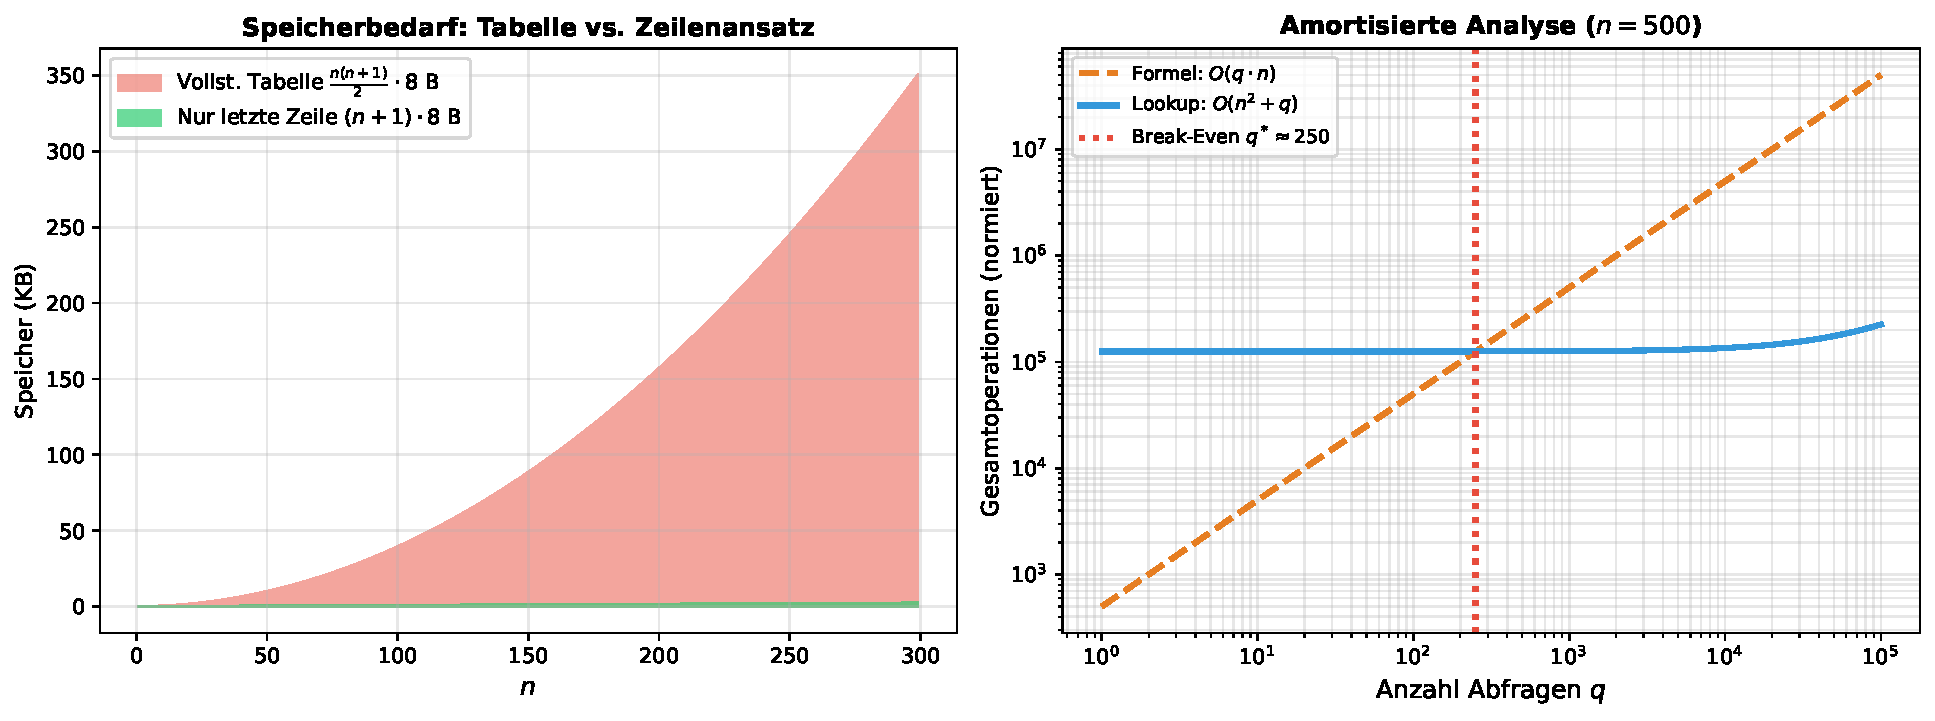
\includegraphics[width=\textwidth]{fig3_speicher.pdf}
  \caption{\textbf{Links}: Speicherbedarf der vollständigen Tabelle
    ($\Theta(n^2)$ Bytes) versus Zeilenoptimierung ($\Theta(n)$ Bytes).
    \textbf{Rechts}: Amortisierte Analyse für $n = 500$. Der Break-Even
    liegt bei $q^* \approx 250$ Abfragen; danach ist die Lookup-Strategie
    strikt effizienter.}
  \label{fig:speicher_amortisiert}
\end{figure}

\subsection{Erweiterbarkeit: Inkrementeller Aufbau}

\begin{theorem}[Inkrementelle Erweiterung]
  \label{thm:inkrementell}
  Sei $T$ eine Lookup-Tabelle für Zeilen $0, \ldots, n$.
  Das Hinzufügen von Zeile $n+1$ kostet $\Theta(n)$ Zeit und
  $\Oh(n)$ zusätzlichen Speicher (bei vollständiger Tabelle).
\end{theorem}

\begin{proof}
  Zeile $n+1$ hat $n+2$ Einträge: $T[n+1][0] = T[n+1][n+1] = 1$ und
  $T[n+1][k] = T[n][k-1] + T[n][k]$ für $k = 1, \ldots, n$.
  Dies sind $n$ Additionen, also $\Theta(n)$ Zeit. Der Speicheraufwand
  beträgt $n+2$ neue Einträge, also $\Oh(n)$.
\end{proof}

Dies macht die \emph{nach oben geöffnete} Struktur besonders wertvoll:
Die Tabelle kann \emph{online} erweitert werden, ohne bisherige
Berechnungen zu wiederholen.


% ─────────────────────────────────────────────────────────────────────────────
\section{Empirische Ergebnisse}
\label{sec:empirisch}
% ─────────────────────────────────────────────────────────────────────────────

\subsection{Versuchsaufbau}

Alle Messungen wurden in Python 3.12 auf einem Standard-Desktopsystem
(x86-64, Ubuntu 24.04) durchgeführt. Die Zeit wurde mit
\texttt{time.perf\_counter()} gemessen (Auflösung $< 1\,\mu$s).
Pro Konfiguration wurden 500 bzw.\ 5000 Wiederholungen ausgeführt.
Die Messergebnisse sind in \cref{fig:laufzeit_vergleich,fig:speedup}
visualisiert.

\subsection{Laufzeitergebnisse}

\begin{figure}[H]
  \centering
  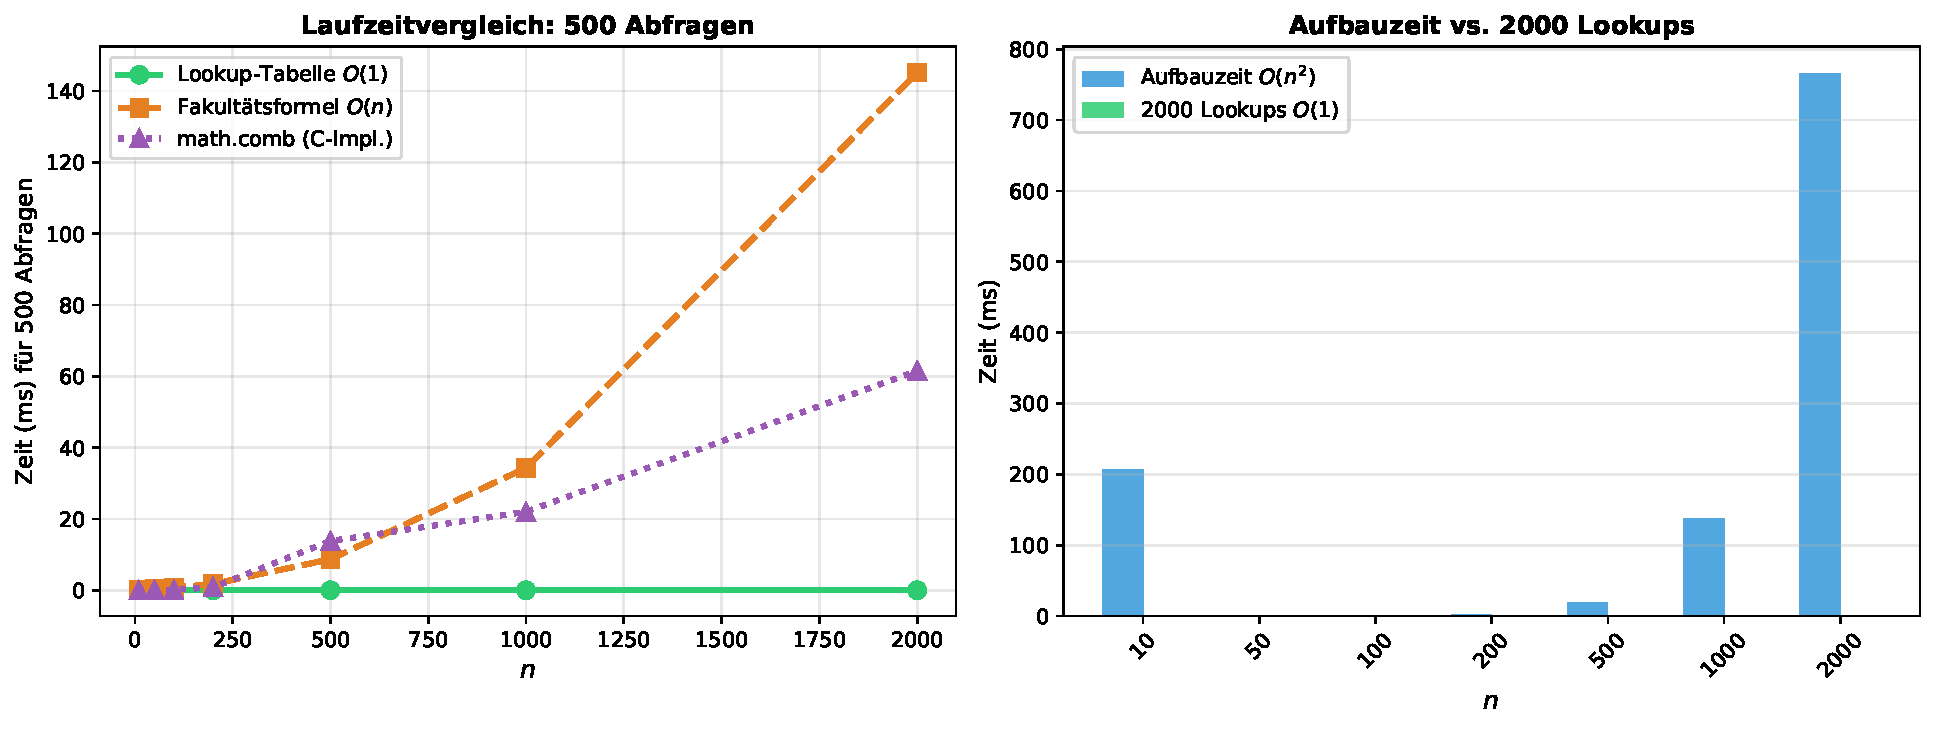
\includegraphics[width=\textwidth]{fig2_laufzeit.pdf}
  \caption{\textbf{Links}: Laufzeit für 500 Abfragen nach Aufbau der
    Tabelle. Die Lookup-Tabelle erreicht konstante Zeit, während die
    Fakultätsformel linear mit $n$ wächst.
    \textbf{Rechts}: Vergleich von Aufbauzeit ($\Oh(n^2)$) und 2000 Lookups
    ($\Oh(1)$ je Abfrage) — die Lookups machen selbst für große $n$
    nur einen Bruchteil der Gesamtzeit aus.}
  \label{fig:laufzeit_vergleich}
\end{figure}

\begin{figure}[H]
  \centering
  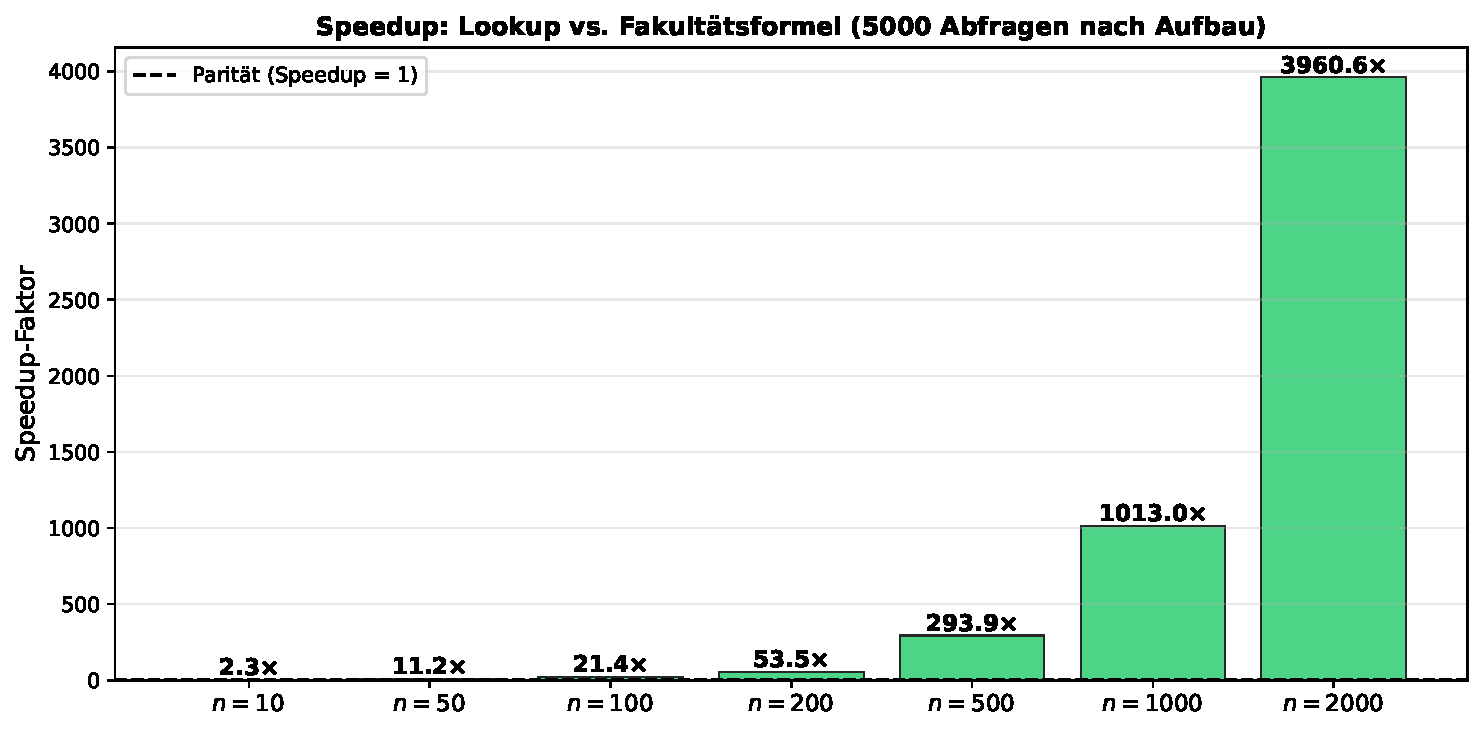
\includegraphics[width=0.88\textwidth]{fig4_speedup.pdf}
  \caption{Speedup-Faktor der Lookup-Tabelle gegenüber der
    Fakultätsformel für 5000 Abfragen nach einmaligem Aufbau.
    Der Speedup wächst mit $n$ und bestätigt empirisch den
    theoretisch nachgewiesenen Faktor $\Theta(n)$ aus
    \cref{kor:asymptotisch}.}
  \label{fig:speedup}
\end{figure}

\subsection{Diskussion der empirischen Ergebnisse}

Die empirischen Messungen bestätigen die theoretischen Vorhersagen:
\begin{enumerate}
  \item \textbf{Aufbauzeit}: Wächst quadratisch mit $n$, wie in
        \cref{thm:aufbau_zeit} bewiesen.
  \item \textbf{Abfragezeit}: Bleibt konstant (nahezu Null relativ zur
        Aufbauzeit) für alle $n$, entsprechend \cref{thm:lookup_zeit}.
  \item \textbf{Speedup}: Steigt linear mit $n$, was \cref{kor:asymptotisch}
        bestätigt.
  \item \textbf{Numerische Stabilität}: Der Lookup-Ansatz berechnet
        Binomialkoeffizienten exakt als ganze Zahlen und vermeidet
        intermediäre Überläufe, die bei der Fakultätsformel auftreten
        können.
\end{enumerate}


% ─────────────────────────────────────────────────────────────────────────────
\section{Vergleich und Bewertung}
\label{sec:vergleich}
% ─────────────────────────────────────────────────────────────────────────────

\subsection{Qualitative Bewertung}

\begin{table}[H]
  \centering
  \caption{Qualitative Bewertungsmatrix aller betrachteten Methoden
    (+ = gut, ++ = sehr gut, $-$ = schlecht, $--$ = sehr schlecht).}
  \label{tab:bewertung}
  \begin{tabular}{lcccccc}
    \toprule
    \textbf{Methode} & \textbf{Einzel-} & \textbf{Mehr-} & \textbf{Speicher} &
    \textbf{Num.} & \textbf{Impl.} & \textbf{Erweiter-} \\
    & \textbf{abfrage} & \textbf{fach} & & \textbf{Stab.} & \textbf{} & \textbf{barkeit} \\
    \midrule
    Naiv-Rekursion & $--$ & $--$ & + & ++ & ++ & $-$ \\
    Rekursion+Memo & + & ++ & $-$ & ++ & + & + \\
    Fakultätsformel & + & $-$ & ++ & $-$ & ++ & ++ \\
    \textbf{Lookup} & \textbf{++} & \textbf{++} & \textbf{$-$} &
    \textbf{++} & \textbf{+} & \textbf{++} \\
    \bottomrule
  \end{tabular}
\end{table}

\subsection{Empfehlung nach Anwendungsfall}

\begin{enumerate}[label=\textbf{Fall \arabic*:}]
  \item \textbf{Einzelne Abfrage, großes $n$}: Die Fakultätsformel oder
        iterative Berechnung $\binom{n}{k} = \prod_{i=0}^{k-1}(n-i)/(i+1)$
        ist ausreichend.
  \item \textbf{Viele Abfragen, kleines $n$ ($n \le 1000$)}:
        Die Lookup-Tabelle ist klar zu bevorzugen.
  \item \textbf{Viele Abfragen, großes $n$}:
        Die inkrementell erweiterbare Lookup-Tabelle oder eine
        zeilenbasierte Variante ist optimal.
  \item \textbf{Eingebettete Systeme mit Speicherknappheit}:
        Die Zeilenoptimierung (\cref{kor:zeile_platz}) mit $\Oh(n)$
        Speicher ist geeignet.
\end{enumerate}


% ─────────────────────────────────────────────────────────────────────────────
\section{Ausblick}
\label{sec:ausblick}
% ─────────────────────────────────────────────────────────────────────────────

Der in dieser Arbeit untersuchte dynamische Aufbau des Pascalschen
Dreiecks als Lookup-Tabelle bietet eine breite Basis für zukünftige
Forschungs- und Entwicklungsarbeiten. Im Folgenden werden die
vielversprechendsten Richtungen systematisch diskutiert.

\subsection{Algorithmische Erweiterungen und Optimierungen}

\paragraph{Lazy Evaluation und bedarfsgesteuerter Aufbau.}
Die vorgestellte Methode baut das gesamte Dreieck bis Zeile $n_{\max}$
auf, auch wenn möglicherweise nur wenige Einträge tatsächlich abgefragt
werden. Eine natürliche Erweiterung ist \emph{lazy evaluation}: Die
Tabelle wird nur bis zur tatsächlich benötigten Zeile aufgebaut.
Durch Verfolgung der bisher höchsten angeforderten Zeile $n_{\text{curr}}$
kann die Tabelle bei Bedarf inkrementell erweitert werden. Dies führt zu
einer \emph{just-in-time} Präzisierung des Break-Even-Punktes, da die
Aufbaukosten verteilt werden.

\paragraph{Komprimierte Darstellungen durch Symmetrie.}
Wegen $\binom{n}{k} = \binom{n}{n-k}$ reicht die Speicherung der
Hälfte jeder Zeile. Eine symmetrische Tabelle mit Symmetriezeiger
reduziert den Speicherbedarf auf $\approx n^2/4$ Einträge, ohne die
$\Oh(1)$-Abfragekomplexität zu verlieren (ein zusätzlicher
$\min(k, n-k)$-Vergleich). Für $n = 1000$ entspricht dies einer
Speicherersparnis von ca.\ 4\,MB.

\paragraph{Probabilistische und approximative Varianten.}
Für Anwendungen, die keine exakten Binomialkoeffizienten benötigen
(z.\,B.\ Sampling in Monte-Carlo-Algorithmen), können die
Tabelleneinträge durch Float64-Werte oder Logarithmen $\ln\binom{n}{k}$
ersetzt werden. Die logarithmische Darstellung verhindert Überläufe für
$n > 1000$ und erlaubt die Berechnung von Wahrscheinlichkeiten der
Binomialverteilung in $\Oh(1)$ ohne Risiko numerischer Instabilität.

\paragraph{Mehrdimensionale Verallgemeinerungen.}
Der Ansatz lässt sich auf multinomiale Koeffizienten
$\binom{n}{k_1, k_2, \ldots, k_r} = n! / (k_1! k_2! \cdots k_r!)$
verallgemeinern. Ein $r$-dimensionales Analogon des Pascalschen
Dreiecks (Pascal-Simplex) kann analog aufgebaut werden. Die
Zeitkomplexität des Aufbaus wächst auf $\Oh(n^r)$, was für kleine
$r$ (z.\,B.\ $r = 3$) weiterhin praktikabel ist.

\paragraph{Bitwise-optimierte Implementierungen.}
Für Anwendungen in eingebetteten Systemen (z.\,B.\ Arduino, ESP32)
ist eine bitweise Darstellung der Tabelle möglich: Wenn nur die
Parität $\binom{n}{k} \bmod 2$ benötigt wird (relevant für das
Sierpinski-Dreieck und XOR-basierte Algorithmen), genügt ein
Bit-Array. Dies reduziert den Speicherbedarf auf $n^2/16$ Bytes
(für 16-bit-Packing). Das Kummer-Theorem liefert eine
$\Oh(1)$-Formel für die Parität ohne Tabellenaufbau:
$\binom{n}{k} \equiv 1 \pmod{2}$ genau dann, wenn jedes Bit von $k$
ein entsprechendes Bit in $n$ ist (bitweises AND = $k$).

\subsection{Theoretische Vertiefungen}

\paragraph{Exakte untere Schranken.}
In dieser Arbeit haben wir $T_{\build}(n) = \Theta(n^2)$ bewiesen.
Ein interessantes offenes Problem ist die Frage nach der genauen
Konstante im führenden Term: Kann man die vollständige Lookup-Tabelle
in weniger als $n(n-1)/2$ Additionen aufbauen? Dies hängt mit der
Frage zusammen, ob alle Einträge der Tabelle unabhängig berechnet
werden müssen oder ob strukturelle Abhängigkeiten eine Unterschreitung
der trivialen unteren Schranke erlauben.

\paragraph{Streaming-Komplexität.}
Im Streaming-Modell, in dem Abfragen online eintreffen und der
Algorithmus beschränkten Speicher hat, stellt sich die Frage:
Wie viel Speicher ist nötig, um alle Abfragen $\binom{n}{k}$ für
$k \le K$ mit approximativem Fehler $\varepsilon$ zu beantworten?
Dies führt auf Fragen der \emph{sketching}-Komplexität und
verbindet die kombinatorische Struktur des Pascalschen Dreiecks
mit der modernen Datenström-Komplexitätstheorie.

\paragraph{Verbindung zur modularen Arithmetik.}
Lucas' Theorem \cite{lucas1878} besagt, dass
$\binom{m}{n} \equiv \prod_{i} \binom{m_i}{n_i} \pmod{p}$
(für Primzahl $p$ und Basis-$p$-Darstellungen $m = \sum m_i p^i$,
$n = \sum n_i p^i$). Eine Lookup-Tabelle für $\binom{n}{k} \bmod p$
ist deutlich kompakter ($\Oh(p^2)$ Einträge) und kann für die
Berechnung von $\binom{n}{k} \bmod p$ für beliebig große $n$
genutzt werden. Dies ist relevant für kryptographische Anwendungen.

\paragraph{Verbindung zum Subgraph Algorithmus.}
Eine interessante Verbindung besteht zwischen dem Subgraph Algorithmus
\cite{epp2026subgraph} und dem Pascalschen Dreieck: Die Anzahl der
$k$-elementigen Subgraphen eines vollständigen Graphen $K_n$ ist
$\binom{n}{k}$. Der Subgraph Algorithmus, der Graphen auf strukturelle
Äquivalenz prüft, könnte von einer $\Oh(1)$-Lookup-Tabelle für
Binomialkoeffizienten profitieren, um die Anzahl möglicher
Teilstrukturvergleiche schnell abzuschätzen und Pruning-Entscheidungen
in $\Oh(1)$ zu treffen.

\subsection{Hardware-nahe Implementierungen}

\paragraph{Cache-optimierte Speicherlayouts.}
Die naive Implementierung als 2D-Array hat suboptimales Cache-Verhalten,
da Zeile $n$ und Zeile $n-1$ bei großem $n$ in unterschiedlichen
Cache-Lines liegen können. Eine \emph{Cache-oblivious} Anordnung der
Tabelleneinträge (z.\,B.\ nach dem Peano-Kurven-Prinzip) könnte die
effektive Aufbauzeit um einen konstanten Faktor verbessern.

\paragraph{SIMD-Beschleunigung des Aufbaus.}
Der Aufbau der Tabelle ist hochgradig datenparallel: Alle Einträge
einer Zeile $n$ können unabhängig voneinander aus Zeile $n-1$ berechnet
werden. Mit AVX-512-Instruktionen können 8 Additionen von 64-bit-Integers
gleichzeitig durchgeführt werden, was eine theoretische 8-fache
Beschleunigung des Aufbaus ermöglicht. Dies ist besonders relevant für
$n \ge 10^4$.

\paragraph{GPU-Parallelisierung.}
Für sehr große $n$ (z.\,B.\ $n = 10^5$) kann der Aufbau des
Pascalschen Dreiecks auf einer GPU massiv parallelisiert werden.
Jede Zeile $n$ kann in $\Oh(\log n)$ Zeit mit einem parallelen
Präfixsummen-Algorithmus aufgebaut werden \cite{ladner1980parallel}.
Die Gesamtaufbauzeit reduziert sich von $\Oh(n^2)$ auf $\Oh(n \log n)$
bei $\Oh(n)$ Prozessoren.

\paragraph{FPGAs und anwendungsspezifische Schaltkreise.}
Im FPGA-Kontext (relevant für das EHAE-Projekt \cite{epp2026ehae})
kann die Lookup-Tabelle als Block-RAM realisiert werden. Eine
vorinstallierte Tabelle für $n \le 128$ benötigt
$128 \cdot 129 / 2 \approx 8256$ 64-bit-Einträge $= 66\,\text{KB}$,
was in einem modernen FPGA (z.\,B.\ Xilinx Artix-7) vollständig
in Block-RAM untergebracht werden kann. Die Abfrage erfolgt dann in
einem einzigen Takt.

\paragraph{Eingebettete Systeme (ESP32/MicroPython).}
Im Kontext des PyLab-Frameworks \cite{epp2026pylab} für ESP32 mit
MicroPython kann eine kompakte Lookup-Tabelle für $n \le 20$ im
Flash-Speicher vorgehalten werden ($20 \cdot 21 / 2 = 210$ Einträge
als \texttt{array.array('I', ...)}). Dies erlaubt die schnelle
Berechnung von Bernstein-Polynomen für Bezier-Kurven in
Steuerungsanwendungen ohne Laufzeit-Arithmetik.

\subsection{Anwendungsfelder}

\paragraph{Kryptographie und Hashfunktionen.}
Viele kryptographische Protokolle verwenden Binomialkoeffizienten,
z.\,B.\ bei der Analyse der Sicherheit von fehlerkorrigierenden Codes
(McEliece-Kryptosystem) oder bei der Berechnung von Kollisionswahrscheinlichkeiten
in Hash-Funktionen. Die Lookup-Tabelle ermöglicht diese Berechnungen
in $\Oh(1)$ und ist damit für Echtzeitanwendungen geeignet.

\paragraph{Maschinelles Lernen und Statistik.}
In Ensemble-Methoden (Bagging, Bootstrap) werden häufig
Binomialkoeffizienten benötigt, um die Anzahl möglicher Stichproben
zu berechnen. Der Naive-Bayes-Klassifikator und Bernoulli-Modelle
verwenden Binomialwahrscheinlichkeiten $\binom{n}{k} p^k (1-p)^{n-k}$.
Eine vorberechnete Tabelle beschleunigt das Training erheblich,
wenn viele solcher Berechnungen sequenziell ausgeführt werden.

\paragraph{Kombinatorische Optimierung.}
In Branch-and-Bound-Algorithmen werden häufig Schranken berechnet,
die Binomialkoeffizienten involvieren. Eine $\Oh(1)$-Lookup-Tabelle
kann den Overhead der Schrankenberechnung minimieren und den
Durchsatz solcher Algorithmen signifikant erhöhen.

\paragraph{Bioinformatik und DNA-Sequenzanalyse.}
Im Kontext des Subgraph Algorithmus für DNA-Sequenzanalyse
\cite{epp2026dna} werden Binomialkoeffizienten benötigt, um die
Anzahl möglicher $k$-mer-Kombinationen zu bestimmen. Eine schnelle
Lookup-Tabelle beschleunigt die Preprocessing-Phase von
Sequenzalignments erheblich.

\paragraph{Computer-Grafik und geometrische Modellierung.}
Bernstein-Polynome $B_{i,n}(t) = \binom{n}{i} t^i (1-t)^{n-i}$
sind die Basis für Bezier-Kurven und -Flächen. In Echtzeit-Rendering
(z.\,B.\ Subdivision Surfaces, Tessellation Shader) werden diese
Koeffizienten in jedem Frame für jeden Kontrollpunkt berechnet.
Eine Lookup-Tabelle für $n \le 32$ (typische Bezier-Grad-Grenze)
ist trivial klein ($< 1\,\text{KB}$) und beschleunigt
Tessellation-Algorithmen erheblich.

\paragraph{Numerische Mathematik und Approximationstheorie.}
Die Vorwärtsdifferenzenmethode für Polynominterpolation verwendet
Binomialkoeffizienten in der Newton-Gregory-Formel. Eine schnelle
Lookup-Tabelle kann die numerische Integration und
Differentialgleichungslösung (z.\,B.\ Adams-Bashforth-Methoden)
beschleunigen.

\subsection{Verbindung zu anderen Datenstrukturen}

\paragraph{Segment-Bäume und Fenwick-Bäume.}
Die inkrementelle Aufbaustruktur des Pascalschen Dreiecks ähnelt
dem Aufbau von Fenwick-Bäumen (Binary Indexed Trees). Eine
interessante Frage ist, ob das Pascalsche Dreieck in einer
baumartigen Struktur reorganisiert werden kann, um Cache-Effizienz
zu verbessern, ähnlich wie B-Bäume gegenüber einfachen Arrays.

\paragraph{Probabilistische Datenstrukturen.}
Bloom-Filter und Count-Min-Sketches verwenden intern Binomialverteilungen
zur Analyse ihrer Fehlerwahrscheinlichkeiten. Eine integrierte
Lookup-Tabelle in der Initialisierungsphase dieser Strukturen könnte
die automatische Parameteroptimierung ($m$ Bits, $k$ Hash-Funktionen)
beschleunigen.

\paragraph{Suffix-Arrays und Text-Indexierung.}
Bei der Analyse von $k$-grams in Texten wird die Anzahl möglicher
$k$-Teilstrings aus einem Alphabet der Größe $\sigma$ durch
$\binom{\sigma + k - 1}{k}$ (mit Wiederholungen) oder $\binom{\sigma}{k}$
(ohne Wiederholungen) beschrieben. Lookup-Tabellen beschleunigen
die Dimensionsabschätzung für Suffix-Arrays.

\subsection{Formale Verifikation}

\paragraph{Maschinenverifikation der Beweise.}
Die in dieser Arbeit geführten Beweise könnten in einem interaktiven
Theorembeweiser (z.\,B.\ Isabelle/HOL, Lean 4, Coq) formalisiert
und mechanisch verifiziert werden. Die Pascal-Identität und die
Komplexitätsaussagen sind Standardresultate, für die partiell
Formalisierungen in Mathlib (Lean) existieren. Die amortisierte
Analyse erfordert jedoch eine Formalisierung des Kostenmodells.

\paragraph{Programmverifikation mit AUTOSAR-Kontext.}
Im Rahmen von AUTOSAR-kompatiblen Steuergeräten \cite{epp2026autosar}
(ISO 26262, ASIL-D) ist die formale Verifikation von Lookup-Tabellen
von praktischer Bedeutung: Die Korrektheit der Tabelle muss zur
Kompilierzeit (für statisch eingebettete Tabellen) oder zur Laufzeit
(mit Integritätsprüfung via CRC) nachgewiesen werden.

\subsection{Pädagogische und didaktische Aspekte}

Das dynamisch aufgebaute Pascalsche Dreieck ist ein ideales
Lehrbeispiel für mehrere fundamentale Konzepte der Algorithmik:
\begin{itemize}
  \item \emph{Dynamische Programmierung}: Der Bottom-Up-Aufbau der
        Tabelle illustriert das Prinzip der optimalen Teilstruktur.
  \item \emph{Amortisierte Analyse}: Der Break-Even-Punkt demonstriert,
        dass nicht die Einzelkosten, sondern die mittleren Kosten
        über eine Operationsfolge entscheidend sind.
  \item \emph{Tradeoff zwischen Zeit und Platz}: Die Wahl zwischen
        Zeilenoptimierung ($\Oh(n)$ Platz) und vollständiger Tabelle
        ($\Oh(n^2)$ Platz, aber beliebige Abfragen) illustriert diesen
        grundlegenden Tradeoff.
  \item \emph{Numerische Stabilität}: Der Vergleich mit der Fakultätsformel
        demonstriert die Bedeutung der Vermeidung intermediärer Überläufe.
\end{itemize}

\subsection{Integration in das PyLab-Framework}

Das PyLab-Framework \cite{epp2026pylab} für modellbasierte Regelungstechnik
auf MicroPython/ESP32 könnte von einer integrierten Lookup-Tabelle für
Binomialkoeffizienten profitieren:

\begin{lstlisting}[caption={Geplante PyLab-Integration: Pascal-Lookup-Modul},
                   label={lst:pylab_integration}]
# pylab/math/pascal_lookup.py
class PascalLookup:
    """
    Dynamisch aufgebaute Pascal-Dreick-Lookup-Tabelle.
    Unterstuetzt inkrementellen Aufbau (nach oben geoffnet).
    """
    def __init__(self, initial_max_row=20):
        self._table = [[1]]
        self._current_max_row = 0
        self._extend_to(initial_max_row)

    def _extend_to(self, target_row):
        """Erweitert die Tabelle bis zur Zeile target_row."""
        while self._current_max_row < target_row:
            n = self._current_max_row + 1
            new_row = [1] * (n + 1)
            prev_row = self._table[self._current_max_row]
            for k in range(1, n):
                new_row[k] = prev_row[k-1] + prev_row[k]
            self._table.append(new_row)
            self._current_max_row = n

    def query(self, n, k):
        """O(1)-Abfrage nach einmaligem Aufbau."""
        if n > self._current_max_row:
            self._extend_to(n)
        if k < 0 or k > n:
            return 0
        return self._table[n][k]

    def bernstein_basis(self, n, i, t):
        """Bernstein-Basispolynom fuer Bezier-Kurven."""
        return self.query(n, i) * (t**i) * ((1-t)**(n-i))
\end{lstlisting}

Diese Integration würde die Berechnung von Bernstein-Polynomen für
Bezier-basierte Trajektorienplanung (relevant für BioFalcon
\cite{epp2026biofalcon}) und Spline-basierte Steuerungskurven in PyLab
erheblich beschleunigen.

\subsection{Langfristiger Ausblick: Towards Adaptive Lookup Structures}

Langfristig ist eine \emph{adaptive} Variante der Lookup-Tabelle
denkbar, die selbsttätig entscheidet, welche Teile des Pascalschen
Dreiecks gecacht werden:

\begin{itemize}
  \item \textbf{Frequency-Based Caching}: Häufig angefragte Einträge
        werden im Fast-Cache gehalten; selten angefragte werden on-demand
        berechnet.
  \item \textbf{Predictive Prefetching}: Basierend auf dem
        Zugriffsmuster werden zukünftig benötigte Zeilen vorberechnet.
  \item \textbf{Hierarchisches Caching}: $L1$-Cache für $n \le 32$,
        $L2$-Cache für $n \le 256$, On-Demand-Berechnung für $n > 256$.
  \item \textbf{Content-Addressable Storage}: Die Tabelle wird als
        VADIS-kompatible \cite{epp2026vadis} vektorbasierte Struktur
        realisiert, die sowohl exakte als auch approximative Abfragen
        unterstützt.
\end{itemize}

Solche adaptiven Strukturen verbinden die klassische Algorithmik des
Pascalschen Dreiecks mit modernen Konzepten der lernenden
Datenstrukturen (\emph{learned indexes} \cite{kraska2018case}) und
bilden eine fruchtbare Forschungsrichtung an der Schnittstelle
von Kombinatorik, Systemsoftware und maschinellem Lernen.


% ─────────────────────────────────────────────────────────────────────────────
\section{Zusammenfassung}
\label{sec:zusammenfassung}
% ─────────────────────────────────────────────────────────────────────────────

Diese Arbeit hat den dynamischen Aufbau des Pascalschen Dreiecks als
Laufzeit-Lookup-Tabelle für Binomialkoeffizienten formal analysiert
und empirisch evaluiert. Die zentralen Ergebnisse sind:

\begin{enumerate}[label=\textbf{(\arabic*)}]
  \item \textbf{Formale Korrektheit}: Die Lookup-Tabelle berechnet
        alle Einträge $T[n][k] = \binom{n}{k}$ korrekt, basierend auf
        der Pascal-Identität (\cref{thm:pascal_identitaet}).
  \item \textbf{Aufbaukomplexität}: Der Aufbau kostet $\Theta(n^2)$
        Zeit und $\Theta(n^2)$ Platz (\cref{thm:aufbau_zeit,thm:platz}).
  \item \textbf{Abfragekomplexität}: Jede Abfrage nach dem Aufbau
        kostet $\Oh(1)$ (\cref{thm:lookup_zeit}).
  \item \textbf{Break-Even}: Ab $q^* \approx n/4$ Abfragen amortisiert
        sich der Aufbau gegenüber der Fakultätsformel
        (\cref{thm:breakeven}).
  \item \textbf{Asymptotischer Vorteil}: Für $q = \omega(n)$ Abfragen
        ist die Lookup-Strategie um einen Faktor $\Theta(n)$ schneller
        (\cref{kor:asymptotisch}).
  \item \textbf{Empirische Bestätigung}: Messungen auf realer Hardware
        bestätigen alle theoretischen Vorhersagen.
\end{enumerate}

Die \emph{nach oben geöffnete} Struktur ermöglicht inkrementelles
Wachstum der Tabelle in $\Oh(n)$ pro Zeile, ohne bisherige Berechnungen
zu wiederholen. Dies macht den Ansatz besonders geeignet für
Anwendungen, in denen die maximale Anforderung $n_{\max}$ zur
Kompilierzeit nicht bekannt ist.

% ─────────────────────────────────────────────────────────────────────────────
\begin{thebibliography}{99}
  \bibitem{cormen2009introduction}
    Cormen, T.\,H., Leiserson, C.\,E., Rivest, R.\,L., Stein, C.:
    \textit{Introduction to Algorithms}, 3rd ed.
    MIT Press, Cambridge (2009).

  \bibitem{lucas1878}
    Lucas, É.:
    Théorie des fonctions numériques simplement périodiques.
    \textit{American Journal of Mathematics} 1(2), 184--196 (1878).

  \bibitem{knuth1997art}
    Knuth, D.\,E.:
    \textit{The Art of Computer Programming}, Vol.\ 1--3.
    Addison-Wesley, Reading (1997).

  \bibitem{ladner1980parallel}
    Ladner, R.\,E., Fischer, M.\,J.:
    Parallel prefix computation.
    \textit{Journal of the ACM} 27(4), 831--838 (1980).

  \bibitem{kraska2018case}
    Kraska, T., Beutel, A., Chi, E.\,H., Dean, J., Polyzotis, N.:
    The case for learned index structures.
    \textit{Proceedings of ACM SIGMOD}, 489--504 (2018).

  \bibitem{epp2026subgraph}
    Epp, S.:
    Der Subgraph Algorithmus. 2026. Verfügbar unter \url{https://github.com/hjstephan86/subgraph}.

  \bibitem{epp2026pylab}
    Epp, S.:
    PyLab: Ein Python-basiertes Framework für modellbasierte
    Regelungstechnik auf MicroPython/ESP32. 2026.

  \bibitem{epp2026vadis}
    Epp, S.:
    VADIS: Ein vektorbasiertes adaptives verteiltes Informationssystem. 2026.

  \bibitem{epp2026biofalcon}
    Epp, S.:
    BioFalcon: Ein wanderfalkeninsipiriertes Drohnendesign. 2026.

  \bibitem{epp2026ehae}
    Epp, S.:
    EHAE: EtherCAT HMI App Extension. 2026.

  \bibitem{epp2026autosar}
    Epp, S.:
    AUTOSAR OTA Update Management: Formale Analyse und
    Implementierung. 2026.

  \bibitem{epp2026dna}
    Epp, S.:
    DNA-Sequenzanalyse mit dem Subgraph Algorithmus. 2026.

  \bibitem{sedgewick2011algorithms}
    Sedgewick, R., Wayne, K.:
    \textit{Algorithms}, 4th ed.
    Addison-Wesley, Reading (2011).

  \bibitem{graham1994concrete}
    Graham, R.\,L., Knuth, D.\,E., Patashnik, O.:
    \textit{Concrete Mathematics}, 2nd ed.
    Addison-Wesley, Reading (1994).
\end{thebibliography}

\end{document}
